\begin{center}
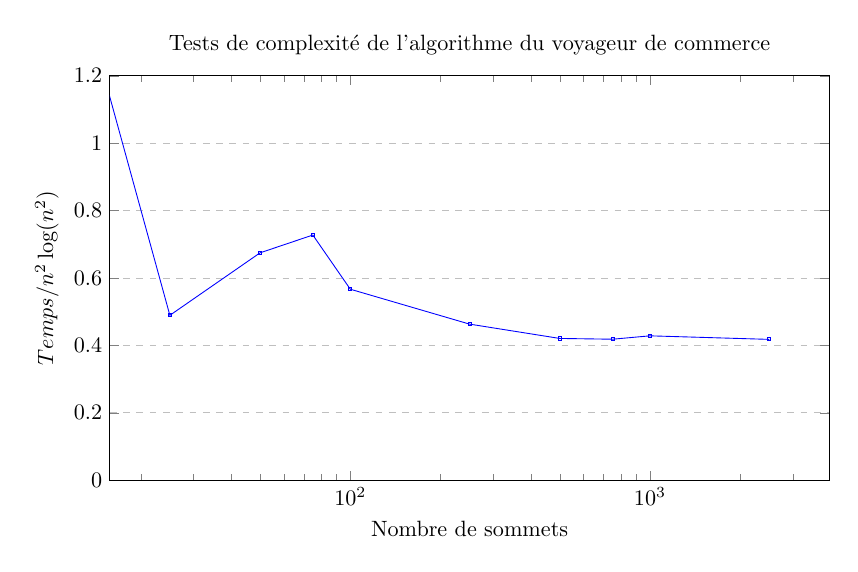
\begin{tikzpicture}[scale=0.8]
\begin{axis}[
    title={Tests de complexité de l'algorithme du voyageur de commerce},
    xlabel={Nombre de sommets},
    ylabel={$Temps/n^{2}\log (n^{2})$},
    ymin=0,ymax=1.2,
    legend pos=north west,
    ymajorgrids=true,
    grid style=dashed,
	xmode=log,
	width=13cm,
	height=8cm
]
 
\addplot[
    color=blue,
	mark=square,
	mark size=0.7
    ]
    coordinates {
		(10,1.77607697441749)(25,0.489248569971374)(50,0.674715987076205)(75,0.727514442260125)(100,0.566688966837445)(250,0.463100665066087)(500,0.420567780829908)(750,0.418296086135812)(1000,0.428329560230366)(2500,0.417812913849976)
	};
 
\end{axis}
\end{tikzpicture}
\end{center}
